\documentclass{article}

\usepackage[a4paper,left=2cm,right=2cm,top=2cm,bottom=1cm,footskip=.5cm]{geometry}

\usepackage{fontspec}
\setmainfont{CMU Serif}
\setsansfont{CMU Sans Serif}
\setmonofont{CMU Typewriter Text}

\usepackage[russian]{babel}

\usepackage{mathtools}
\usepackage{karnaugh-map}
\usepackage{tikz}
\usetikzlibrary{circuits.logic.IEC}
\usepackage[table]{xcolor}
\usepackage{graphicx}

\begin{document}

%=============== Титульный лист ===============%
\begin{center}
    УНИВЕРСИТЕТ ИТМО \\
    Факультет программной инженерии и компьютерной техники \\
    Дисциплина «Дискретная математика»
    
    \vspace{5cm}
    
    \large
    \textbf{Курсовая работа} \\
    Нечёткий вывод по схеме Мамдани
\end{center}

\vspace{10cm}

\hfill\begin{minipage}{0.35\linewidth}
Выполнил \\
Горин Семён Дмитриевич \\
P3108 \\

Преподаватель \\
Поляков Владимир Иванович
\end{minipage}

\vfill

\begin{center}
    Санкт-Петербург, 2025 г.
\end{center}

\thispagestyle{empty}
\newpage

%=============== Содержание ===============%
\tableofcontents
\newpage

%=============== Содержательная постановка задачи ===============%
\section{Содержательная постановка задачи}

\textbf{Задача:} разработать алгоритм нечеткого вывода по схеме «Мамдани», по которому определяется, сколько баллов БаРС набрал студент за семестр, исходя из его посещаемости занятий и средней оценки за тесты.

\medskip

\textbf{Входные данные:}
\begin{enumerate}
    \item Посещенные занятия (в академических часах) $h \in [0;32]$.
    \item Усредненная оценка за тесты $y \in [2;5]$.
\end{enumerate}

\textbf{Выходные данные:} количество баллов БаРС (в баллах) $z \in [0;103]$.

%=============== Шаг 1. Фазификация ===============%
\section{Фазификация}

Во входных данных заданы две переменные:
\begin{itemize}
    \item $h$ — число посещённых академических часов ($0 \le h \le 32$).
    \item $y$ — усредненная оценка за тесты ($2 \le y \le 5$).
\end{itemize}

Необходимо разбить каждую из этих переменных на лингвистические термы и определить для них функции принадлежности.

\subsection{Лингвистические термы для посещаемости $h$}

\begin{itemize}
    \item \textbf{LA} (Low Attendance) — низкая посещаемость.
    \item \textbf{MA} (Medium Attendance) — средняя посещаемость.
    \item \textbf{HA} (High Attendance) — высокая посещаемость.
\end{itemize}

Функции принадлежности: 

\begin{align*}
\mu_{LA}(h) = \dfrac{11 -h}{11}, &\quad 0 \le h \le 11
\end{align*}

\[
\mu_{MA}(h) =
\begin{cases}
\dfrac{h - 10}{6}, & 10 \le h \le 16,\\
\dfrac{22 - h}{6}, & 16 \le h \le 22
\end{cases}
\]
\begin{align*}
\mu_{HA}(h) = \dfrac{h - 21}{11}, &\quad 21 \le h \le 32
\end{align*}

%-------- График функций для h --------%
\begin{figure}[h!]
    \centering
    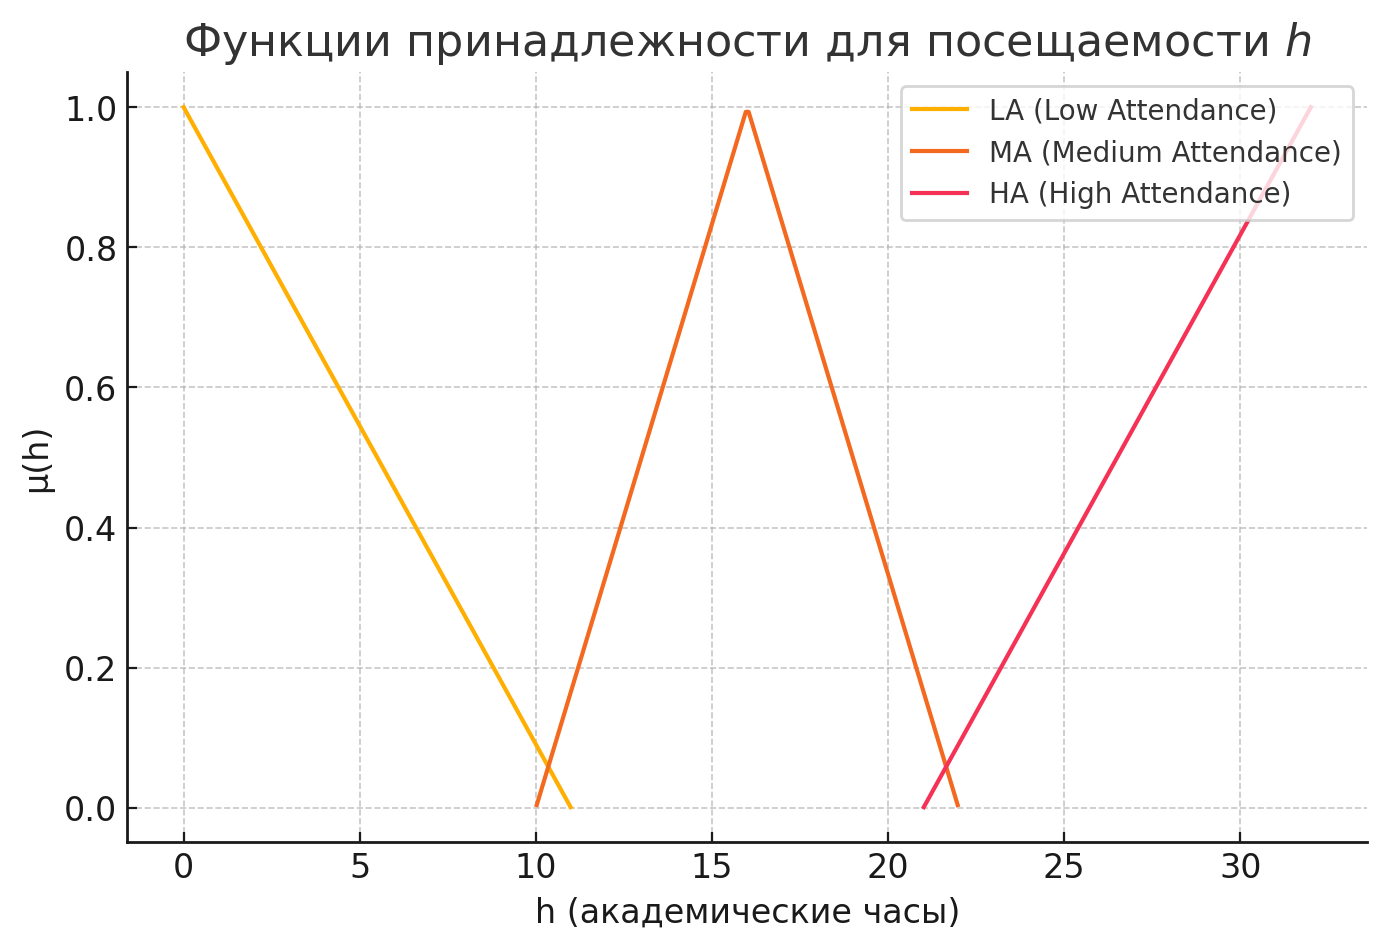
\includegraphics[width=0.8\linewidth]{membership_h.png}
    \caption{Функция принадлежности для посещаемости $h$.}
    \label{fig:membership_h}
\end{figure}

\newpage
\subsection{Лингвистические термы для средней оценки $y$}

\begin{itemize}
    \item \textbf{LAS} (Low Average Score) — низкая средняя оценка.
    \item \textbf{MAS} (Medium Average Score) — средняя усреднённая оценка.
    \item \textbf{HAS} (High Average Score) — высокая средняя оценка.
\end{itemize}

Функции принадлежности:
\begin{align*}
\mu_{LAS}(y) = 1 - \dfrac{y - 2}{1}, & 2 \le y \le 3
\end{align*}
\[
\begin{cases}
\mu_{MAS}(y) =
\dfrac{y - 2.5}{1}, & 2.5 \le y \le 3.5,\\
1 - \dfrac{y - 3.5}{1}, & 3.5 \le y \le 4.5\\
\end{cases}
\]

\begin{align*}
\mu_{HAS}(y) = \dfrac{y - 3.5}{1.5}, & 3.5 \le y \le 5
\end{align*}




%-------- График функций для y --------%
\begin{figure}[h!]
    \centering
    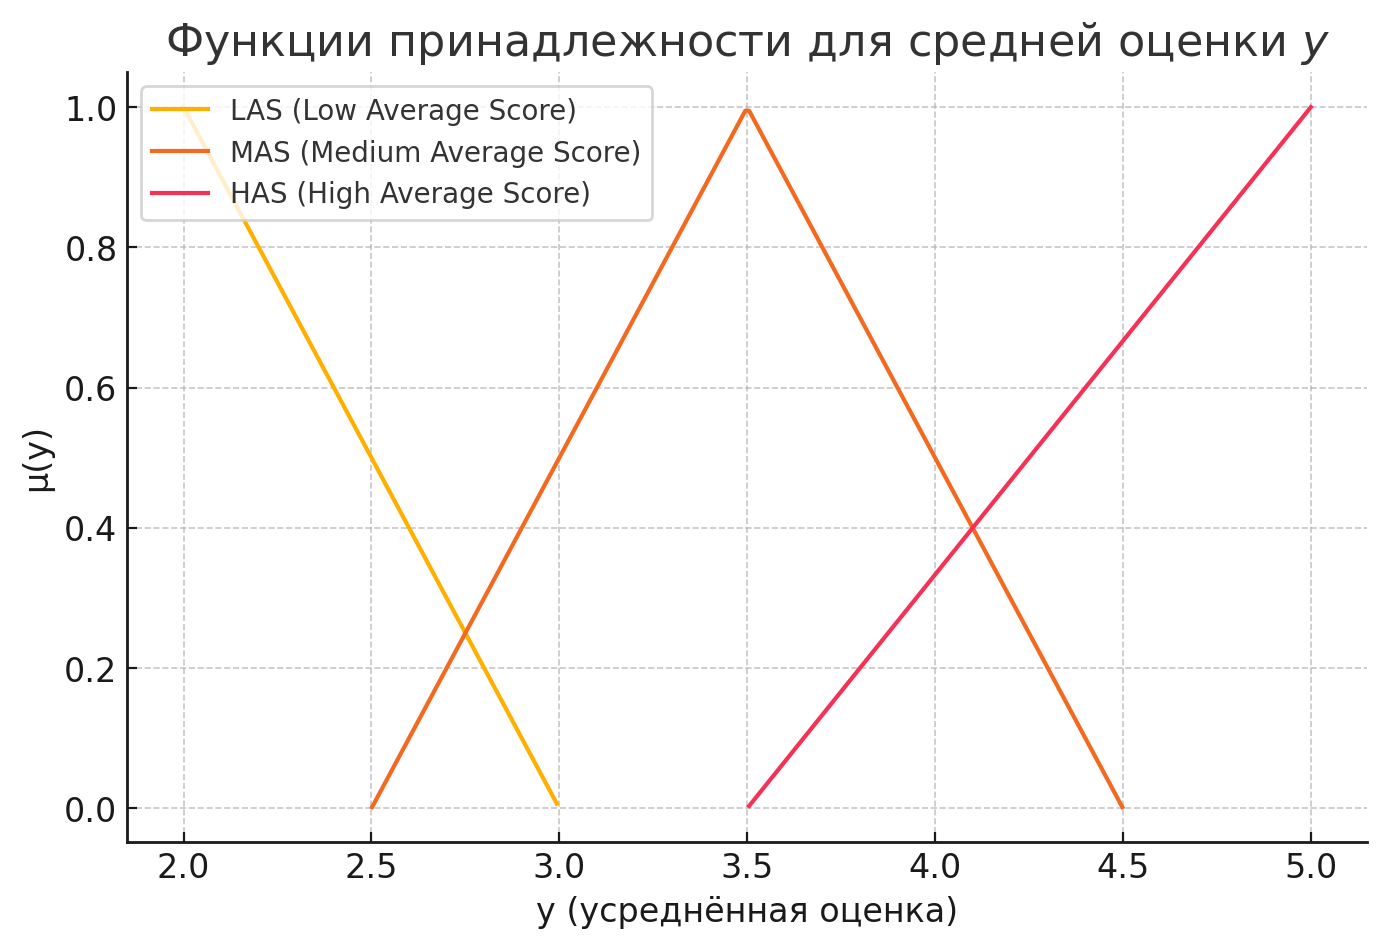
\includegraphics[width=0.8\linewidth]{membership_y.png}
    \caption{Функция принадлежности для оценки $y$.}
    \label{fig:membership_y}
\end{figure}

\newpage
\subsection{Лингвистические термы для выходной переменной $z$}

Выходная переменная $z$ (количество баллов БаРС) лежит в диапазоне $[0;103]$. Разобьём её на пять термов:
\begin{itemize}
    \item \textbf{PS} (Puny Score) — ничтожное количество баллов.
    \item \textbf{LS} (Low Score) — малое количество баллов.
    \item \textbf{MS} (Medium Score) — среднее количество баллов.
    \item \textbf{HS} (High Score) — высокое количество баллов.
    \item \textbf{OS} (Outstanding Score) — очень высокое количество баллов.
\end{itemize}

Функции принадлежности:
\begin{align*}
    \mu_{PS}(z) = 1 - \dfrac{z}{20}, & 0 \le z \le 20
\end{align*}

\[
\mu_{LS}(z) =
\begin{cases}
\dfrac{z - 10}{15}, & 10 \le z \le 25,\\
1 - \dfrac{z - 25}{15}, & 25 \le z \le 40,\\
\end{cases}
\]
\[
\mu_{MS}(z) =
\begin{cases}
\dfrac{z - 30}{20}, & 30 \le z \le 50,\\
1 - \dfrac{z - 50}{20}, & 50 \le z \le 70,\\
\end{cases}
\]
\[
\mu_{HS}(z) =
\begin{cases}
\dfrac{z - 60}{15}, & 60 \le z \le 75,\\
1 - \dfrac{z - 75}{15}, & 75 \le z \le 90,\\
\end{cases}
\]
\begin{align*}
    \mu_{OS}(z) = \dfrac{z - 80}{23}, & 80 \le z \le 103    
\end{align*}



%-------- График функций для z --------%
\begin{figure}[h!]
    \centering
    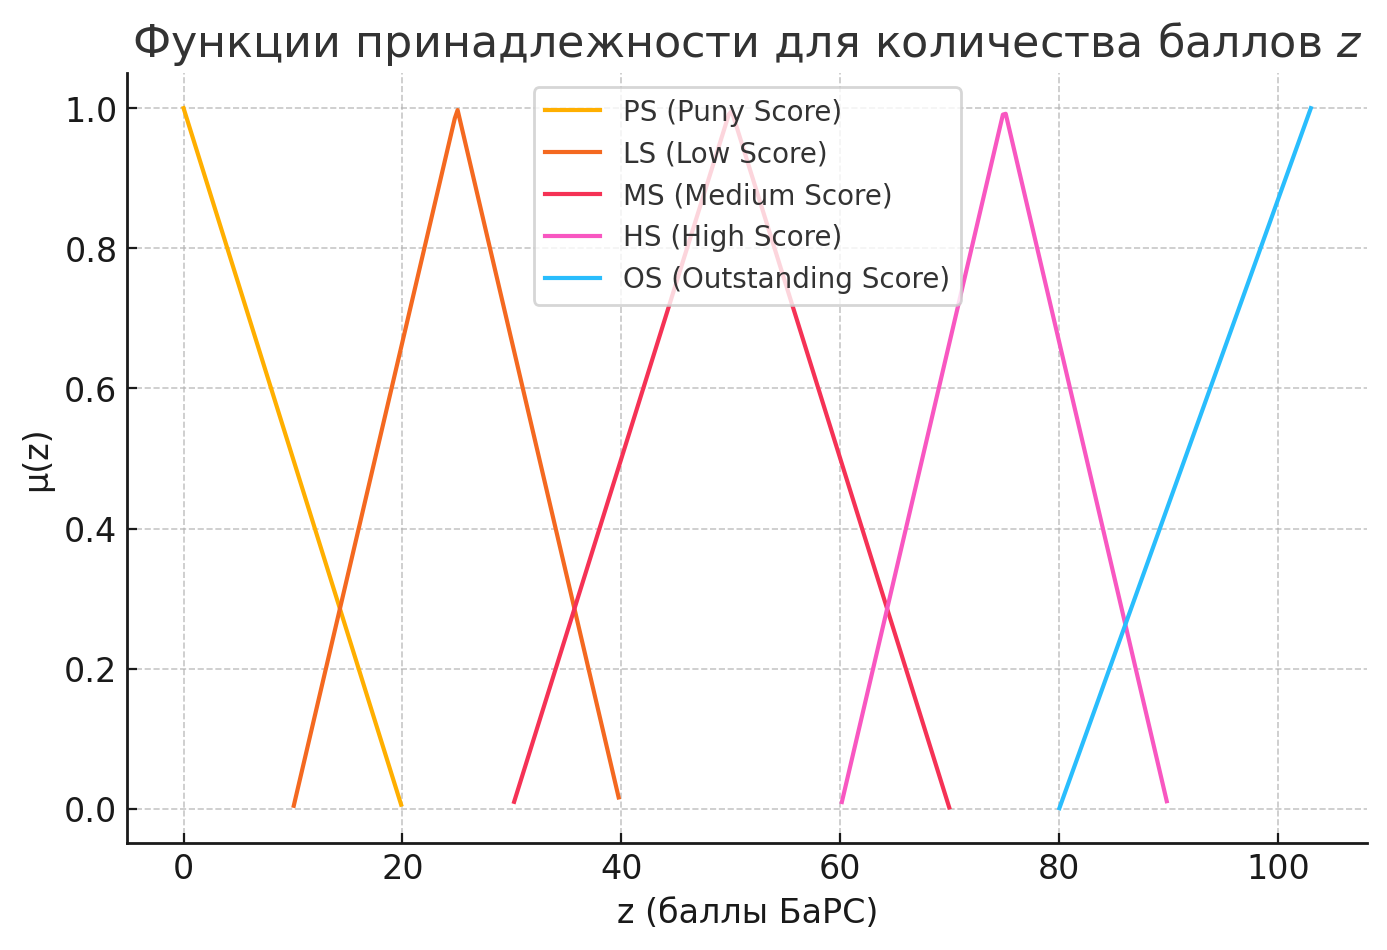
\includegraphics[width=0.8\linewidth]{membership_z.png}
    \caption{Функция принадлежности для выхода $z$.}
    \label{fig:membership_z}
\end{figure}

\newpage
%=============== Шаг 2. Блок выработки решения ===============%
\section{Блок выработки решения}

На основе лингвистических термов построим базу правил

\begin{center}
\begin{tabular}{|c|c|c|c|}
\hline
\multicolumn{1}{|c|}{\textbf{Посещаемость $\backslash$ Средняя оценка}} & \textbf{LAS} & \textbf{MAS} & \textbf{HAS} \\ \hline
\textbf{LA}   & PS   & LS   & MS   \\ \hline
\textbf{MA}  & LS   & MS   & HS   \\ \hline
\textbf{HA}  & MS   & HS   & OS   \\ \hline
\end{tabular}
\end{center}

\bigskip

\subsection{Процедура вычисления истинности правил}

Пусть заданы входные значения
\[
  h = 25,\quad y = 4.0.
\]
Вычислим сразу ненулевые степени принадлежности:
\[
  \mu_{HA}(25) \;=\; \frac{25 - 21}{11} \;=\; 0.364,\qquad
  \mu_{MAS}(4.0) = 0.50,\qquad
  \mu_{HAS}(4.0) \approx 0.333.
\]
\medskip

\begin{center}
\renewcommand{\arraystretch}{1.3}% чуть увеличим высоту строк
\begin{tabular}{|c|c|c|c|}
\hline
\rowcolor{gray!20}
\multicolumn{1}{|c|}{\textbf{Посещаемость\,/\,Средняя оценка}} 
  & \textbf{LAS} & \textbf{MAS} & \textbf{HAS} \\ \hline

\rowcolor{white}
\textbf{LA} 
  & PS & LS & MS \\ \hline

\rowcolor{white}
\textbf{MA} 
  & LS & MS & HS \\ \hline

\rowcolor{white}
\textbf{HA} 
  & MS 
  & \cellcolor{green!30}\textbf{HS} 
  & \cellcolor{green!30}\textbf{OS} \\ \hline
\end{tabular}
\end{center}

\medskip


Для каждой из этих двух активированных ячеек вычисляем степень истинности:\\
Аггрегирование:
\[
  \alpha_{\mathrm{HS}} 
  = \min\bigl(\mu_{HA}(25),\,\mu_{MAS}(4.0)\bigr) 
  = \min(0.364,\,0.50) = 0.364
\]
\[
  \alpha_{\mathrm{OS}} 
  = \min\bigl(\mu_{HA}(25),\,\mu_{HAS}(4.0)\bigr) 
  = \min(0.364,\,0.333) = 0.333.
\]

Активация:
\[
  \tilde\mu_{HS}(z) = \min\bigl(\mu_{HS}(z),\,0.364\bigr), 
  \qquad
  \tilde\mu_{OS}(z) = \min\bigl(\mu_{OS}(z),\,0.333\bigr),
\]
Аккумулирование:
\[
  \mu_{\mathrm{agg}}(z) 
  \;=\; 
  \max\bigl(\tilde\mu_{HS}(z),\,\tilde\mu_{OS}(z)\bigr),
  \quad z\in [0,\,103].
\]



%=============== Шаг 3. Дефазификация ===============%
\section{Дефазификация}

Для получения единственного числового ответа \(z^*\) применяем метод центра тяжести:
\[
  z^* 
  \;=\; 
  \frac{\displaystyle \int_{0}^{103} z\,\mu_{\mathrm{agg}}(z)\,dz}
       {\displaystyle \int_{0}^{103} \mu_{\mathrm{agg}}(z)\,dz}.
\]
При численной аппроксимации получаем 
\[
  z^* \approx 82.4.
\]
Таким образом, при \(h=25\) и \(y=4.0\) студент набирает примерно \(82\) балла БаРС.


\end{document}
